\documentclass[journal]{IEEEtran}
\usepackage{amsmath,amsfonts}
\usepackage{algorithmic}
\usepackage{algorithm}
\usepackage{alphabeta}
\usepackage{array}
\usepackage[caption=false,font=scriptsize,labelfont=sf,textfont=sf]{subfig}
\usepackage{textcomp}
\usepackage{stfloats}
\usepackage{url}
\usepackage{verbatim}
\usepackage{graphicx}
\usepackage{cite}
\usepackage{listings}
\hyphenation{op-tical net-works semi-conduc-tor IEEE-Xplore}

\begin{document}

\title{Advanced Signal Processing for Solid State Nanopores}
\author{Soham Gokhale,\ el22sag@leeds.ac.uk,\ Dr. Paolo Actis (Supervisor), Dr. John Cunningham (Assessor)}

\markboth{ELEC5882 MSc Individual Project 2022/23, University of Leeds}{}

\maketitle

\begin{abstract}
Placeholder for abstract
\end{abstract}

\begin{IEEEkeywords}
Sample Keywords
\end{IEEEkeywords}

\section{Introduction}
\IEEEPARstart{A}{}biological cell contains tiny channels through which it exchanges various molecules and ions with the outside world. These channels are typically nanometre sized holes present on the thin walls of the cell membrane. Studying the passage of molecules through such small channels or nanopores can possibly reveal information about their characteristics. Over the past few decades, scientists have been able to develop various techniques to artificially fabricate such nanopores using solid state materials \cite{dekkerSolidstateNanopores2007,xueSolidstateNanoporeSensors2020}. Nanopore sensors have found many applications such as study of bio-molecules, behaviour of nano-particles, analysis of proteins \cite{luoApplicationSolidStateNanopore2020} and DNA Sequencing \cite{deamerThreeDecadesNanopore2016}. Solid state nanopore sensors work on the principle of temporary ionic current blockage across a pore at a given voltage bias. Whenever a molecule passes through a nanopore it disrupts the current path inducing sudden changes in the ionic current. These are known as translocation events. The translocation events can reveal lot of information about the analyte molecule. By analysing the various features of this signal such as amplitude, event duration etc., it is possible to infer the characteristics of the analyte \cite{wenGuideSignalProcessing2021}.

A typical setup for solid-state nanopore sensing involves a thin non-permeable membrane containing a nanopore. This membrane is immersed in an electrolytic bath usually filled with buffered salt solution. Two electrodes are placed on each side of the membrane to induce voltage bias which causes ionic current to flow. This current is measured using highly sensitive measuring instruments to monitor fluctuations. During translocation events, this current is blocked proportional to the blockage of the nanopore. Different analytes may interact differently with the ions causing changes in the current flow \cite{xueSolidstateNanoporeSensors2020}.

The signal generated by solid-state nanopores is of very small amplitude, typically in pico-ampere to nano-ampere range. The signal is often spread out over a wide range of frequencies. Furthermore, the nature of the signal may change depending upon the analyte material, type of nanopore and composition of the electrolytic bath \cite{gokhaleAdvancedSignalProcessing2023}. For example, the translocation events may appear as current pulses or spikes, short lived changes in the conductance state, or long multi-state changes in the current level \cite{forstaterMOSAICModularSingleMolecule2016,varongchayakulSinglemoleculeProteinSensing2018}. Various solutions have been proposed in order to overcome the limitations of solid state nanopore signals. These involve improved fabrication techniques, improving the physical and electrochemical properties of the nanopores, making the electrolyte solution more conducive to sensing as well as improving the sensing equipment \cite{chauMacromolecularCrowdingEnhances2020,gokhaleAdvancedSignalProcessing2023,milesSingleMoleculeSensing2012}. However, it is clear that signal processing plays a crucial role in analysis of nanopore signals and will help in studying the analytes further \cite{milesSingleMoleculeSensing2012,varongchayakulSinglemoleculeProteinSensing2018}.

\subsection{Aims and Objectives}
Due to the differences in these signals, developing a generalised algorithm for signal processing is a complex task. A robust signal processing software should be able to separate the useful information in the signal from the unwanted noise in order to aid in drawing conclusions about the analyte. It should be able to detect events with good accuracy and it should also have various visualisation tools available in order to properly represent the data in visually intuitive formats.

\noindent \textit{Project Aims}
\begin{enumerate}
\item {The aim of this project is to develop a comprehensive tool that will allow researchers to analyse, process, and visualise nanopore data by employing different signal processing techniques and visualisation tools \cite{gokhaleAdvancedSignalProcessing2023}}
\item {The software must be flexible enough to cater to the distinctive requirements of the various types of nanopore signals.}
\item {Researchers should be able to add new algorithms to the software and test them without having to change existing components or structure of the application.}
\end{enumerate}

\noindent \textit{Project Objectives}
\begin{enumerate}
\item {The software must employ algorithms for signal denoising, baseline detection, detecting translocation events, extracting event features and data visualisation.}
\item {Algorithms used at each processing stage must be swappable without impacting other blocks of the signal chain.}
\item {The signal chain must be dynamically re-arrangeable with provisions to add/remove blocks.}
\end{enumerate}

\section{Literature Review}
In recent decades, there has been a remarkable expansion in the realm of solid-state nanopores with applications across many fields. There has been ground-breaking research in using nanopores for DNA sequencing. Oxford Nanopore technologies have been able to successfully develop commercial nanopore sequencers which are capable of long read lengths and real-time base calling \cite{ipMinIONAnalysisReference2015}. Solid-state nanopores have also shown great promise in the study of other nano-particles and single-molecule analytes such as proteins. As the nanopore signal is heavily influenced by the experimental set-up and the analyte material, each application may have a unique set of signal processing requirements. Several signal processing tools have been developed to cater to various such applications and their needs. Many of these are free and open-source software that can be used by researchers all over the globe for analysing data generated by nanopore experiments.

MOSAIC \cite{forstaterMOSAICModularSingleMolecule2016} and SquiggleKit \cite{fergusonSquiggleKitToolkitManipulating2019} are two signal processing tools which are targeted towards multi-state nanopore signals, such as those generated during nanopore DNA sequencing. Both these are developed using Python programming language. As a denatured DNA molecule passes through a nanopore, each nucleotide exhibits different resistivity across the opening of the pore. This induces different levels of ionic current blockages creating multiple conductance states in the signal. MOSAIC introduced two novel algorithms for the analysis of multi-state signals viz. ADEPT and CUSUM+. Both these algorithms were able to detect previously undetected state changes and short-lived events \cite{forstaterMOSAICModularSingleMolecule2016}.MOSAIC natively supports ‘abf’ and ‘qdf’ file formats which are commonly used to store binary data from biomedical experiments. SquiggleKit on the other hand focuses on ‘fast5’ file format which is used by the nanopore sequencers developed by Oxford Nanopore Technologies. It acts as an interface to process and visualise raw nanopore data. SquiggleKit’s \textit{MotifSeq} algorithm is also capable of DNA base-calling from raw data \cite{fergusonSquiggleKitToolkitManipulating2019}.

Researches at TU Delft in 2015 developed ‘Transalyzer’ which is a Matlab based GUI package for nanopore data analysis \cite{plesaDataAnalysisMethods2015}. Converse to those mentioned before, Transalyzer is more suited for experiments that generate spikes or single conductance state blockages during translocation events. Transalyzer provides highly efficient data analysis methods and algorithms for event detection and characterisation. These include an iterative baseline detection algorithm and a method for detecting small current spikes within translocation events. At its launch, Transalyzer aimed to be a comprehensive tool that combined different algorithms for nanopore data analysis. However, the tool is not actively maintained and has not been able to incorporate newer algorithms \cite{plesaDataAnalysisMethods2015}. Other tools have been developed by different labs across various research institutions across the globe in response to the requirements of their experimental data and objectives such as OpenNanopore developed by EPFL \cite{raillonFastAutomaticProcessing2012}. There are also pay-to-use software packages such as Nanolyzer developed by Northern Nanopore Instruments. Nanolyzer is flexible enough to cater for various types of nanopore data and is actively maintained with new features being added regularly. However, being a paid software limits its accessibility as well as the ability to make your own custom modifications to the software.

All the software tools under consideration exhibit remarkable proficiency when employed on signals that align with their inherent capabilities, yielding outcomes of a notably high standard. Most of them also allow modification and extending their source code to tweak them for specific scenarios. However, these tools have certain assumptions about the type of data for which they can be utilised and have limitation with regards to expanding their capabilities or adding newer algorithms.

\section{Typical Signal Processing Flow}
As shown in Fig. 1, the initial proposed structure of the software application was similar to that typically followed by existing tools. There are four crucial steps to processing nanopore data irrespective of the nature of the signal \cite{forstaterMOSAICModularSingleMolecule2016,gokhaleAdvancedSignalProcessing2023,plesaDataAnalysisMethods2015,wenGuideSignalProcessing2021}. These steps are as follows:

\begin{figure}[!t]
\centering
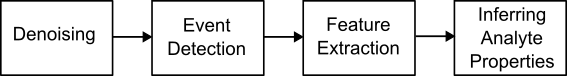
\includegraphics[width=3in]{imgs/TypSigFlow.png}
\caption{Typical Signal Processing Flow for Solid-State Nanopore Data}
\label{fig_1}
\end{figure}

\noindent {\bf{Step 1}}: The raw data contains unwanted noise elements which need to be removed. Typically this is done using filters. This can be achieved using simple low pass Butterworth or Bessel filters or even complex wavelet filters which have better performance \cite{shekarWaveletDenoisingHighBandwidth2019}. Filtering may not be necessary if the signal to noise ratio is sufficiently high \cite{wenGuideSignalProcessing2021}. \\
{\bf{Step 2}}: Once the data is cleaned, the translocation events need to be separated from the signal. This involves identifying spikes and conduction level changes. The exact algorithm used to achieve this might depend on the nature of the signal. Certain preprocessing steps may be required to facilitate the accurate and effective detection of events considering the variety of unique attributes. \\
{\bf{Step 3}}: After isolating the events, various features of each event can be extracted. For single molecule analytes this may include amplitude at maxima, event duration, dwell time (event duration at full width half maximum) etc. For DNA sequencing this may involve base-calling. \\
{\bf{Step 4}}: Inferring properties of the analyte may be a manual process using visualisation tools to represent extracted features. Visualisation can help identify patterns, similarities and distinctions within the data. This process can also be automated by using statistical methods or machine learning algorithms.

The initial design of the software was implemented on MATLAB and was able to generate results of acceptable standards. It utilized Butterworth LPF for denoising, moving window average for baseline detection and amplitude threshold based event detection. Even though baseline detection is not an explicit step in the signal processing flow, it is a crucial step to ensure high accuracy in event detection. Detecting the baseline, subtracting baseline from original signal and in some cases flipping the signal to make sure events are in desired direction (positive spikes or negative spikes) were all included in the event detection phase. This made it difficult to modify the baseline detection algorithm without impacting event detection as the algorithms were tightly coupled and had internal dependencies. There also arose a need for visualisation between many of the steps such as plotting the raw signal and filtered signal to inspect noise levels, visually inspecting individual event traces etc. Thus, it can be noted that even thought the signal processing flow can be categorised broadly into four steps, there can be a need for additional processing in between each step. This demands a flexible structure that cannot be divided into four distinct steps. The PyNanoporeAnalyzer application has been designed with a modular structure in order to overcome the drawbacks of existing software tools.

\section{Software Design}
\subsection{General Architecture}
In order to provide the required flexibility to the signal processing flow, each processing unit is separated into individual blocks. Each of these blocks is designed to execute a specific operation on the input signal. For example a block may perform signal filtering or baseline detection. Having blocks perform isolated tasks makes the application more decoupled, which makes it easier to make additions and modifications. By allowing users to interconnect various blocks, a highly customised signal flow can be constructed to suit specific requirements. This flexible architecture also permits the inclusion of multiple blocks of the same type within the signal chain. 

\begin{figure}[!t]
\centering
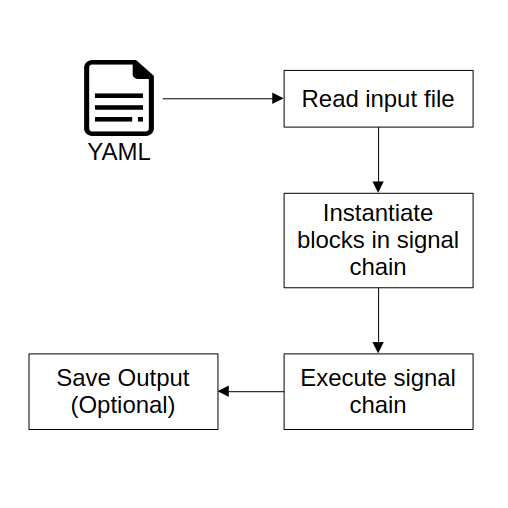
\includegraphics[width=3in]{imgs/SW-Arch.png}
\caption{Software architecture of PyNanoporeAnalyzer}
\label{fig_2}
\end{figure}

Fig. 2 shows the overall architectural framework of the PyNanoporeAnalyzer application. The application begins its execution by reading an input file which is in ‘yaml’ format. The YAML file format is chosen to make the input file human readable and easy to write. This file contains descriptions about each block such as its type, implementation class, inputs, parameters etc. It also contains the connections of each block in the signal chain. The application starts by reading the input file and instantiates the blocks based on the parameters specified in the input file. This phase also sets up the signal chain and determines the signal path. Any validations or checks on the signal chain can also be performed during this phase. Once the signal path is established, the application traverses the signal chain by executing each block one by one. Plots and other visualisation tools are also defined as blocks wherein each block can be used to generate a different figure. These visualisation outputs can also be stored for future reference.
	
The application therefore does not follow a fixed sequence of processing stages. The flow of the signal and the processing performed is determined at run-time based on the descriptions in the input file. This removes the issues associated with a rigid signal processing structure. Using this approach, it is now possible to modularise the sub-functions required at each step making the code reusable and the application more robust in its structure. This modular approach means it is possible to add new algorithms to the existing application with minimum modifications. It is also possible to test the performance of new algorithms and compare them to existing ones in a single signal flow. By separating the initialisation and execution of the blocks, it becomes easier to perform validations on the signal flow parameters. It also ensures these validation are performed before the heavy computational tasks of actual signal processing are commenced. 

\subsection{Structure of a Block}


\begin{figure}[!t]
\centering
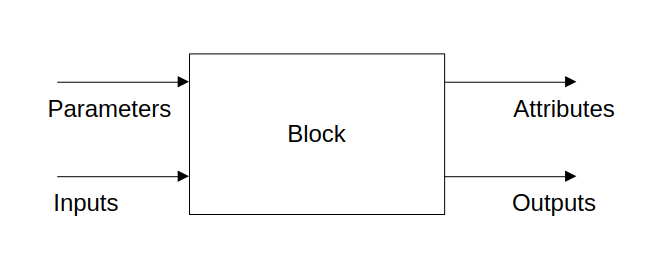
\includegraphics[width=3in]{imgs/Block.png}
\caption{General Structure of a Block}
\label{fig_3}
\end{figure}

All blocks follow a uniform fundamental structure, thereby enabling the application to seamlessly interchange any block within the signal chain. This structure is shown in Fig. 3. Each block has four components - \textit{parameter}, \textit{attributes}, \textit{inputs} and \textit{outputs}. \\
{\bf{Parameters}} are the set of arguments passed to the block during the instantiation phase. The parameters determine the configurations used by the blocks during their execution. For example, parameters to a Butterworth low pass filter block may include the cut-off frequency and order of filter. The exact threshold value to be used for event detection is also an example of a parameter. \\
{\bf{Inputs}} to the block are the set of arguments passed to it during execution. The signal to be processed will almost always be the input to a block. The actual processing will be performed primarily on the inputs of the block. Some blocks may take more then one signals as input to generate the output, one example is to subtract two signals. Inputs may also contain parameters that cannot be provided during instantiation. For example, the parameters dependent upon the output of another block which cannot be known before the execution starts. \\
{\bf{Outputs}} of the block are values returned by the block. Outputs of a block will only contain the processed signal. By having an expected return value type, it becomes easier to rearrange blocks in the signal chain dynamically. However, there may be more than one values generated during a blocks execution. Even in this case only the processed signal is returned as the output. \\
{\bf{Attributes}} are all the internally generated values by a block during its execution. These values may be useful for other blocks for their operation. For example, the event detection block stores the various features of the signal such as event amplitude, dwell time etc. as attributes. These attributes may be taken as input by other blocks.

It is not necessary that all blocks will have parameters, attributes, inputs or outputs. There are four types of blocks in PyNanoporeAnalyzer - \textit{source, process, sink} and \textit{ visualisation}. A \textit{source} blocks that loads data will not have any inputs where the path to data file might be the sole parameter. This type of block will have the extracted signal as its output which can be passed to further blocks for processing. Conversely, block responsible for feature extraction will not have any output as all the processing needs to be ideally done before this step. All the features will be stored as attributes and the block will act as a signal \textit{sink}. Some blocks may even take attributes of other blocks as inputs. Visualisation blocks are good examples of this where they can have the extracted features and not the signal itself as inputs. As a general rule, all blocks involved in signal processing will be of \textit{process} type. The inputs and outputs of such blocks must contain the only the signal while using parameters and attributes for any other data associated with the signal. Visualisation blocks however, can have any data as input as they do not perform any operations on the it directly. This is just a general guideline and the application does not force the user to follow it. However, the application handles the blocks in a slightly different manner depending on the type.

\section{Implementation and Results}
\subsection{Input File}
The input file serves as a description of interconnected signal processing blocks and their configurations within the signal chain. This file is used during runtime to establish and execute the signal processing flow. The input file is in YAML format which is widely used for configuration files. Using this format offers an accessible means for users to construct and modify signal flows as needed. The input file structure is organised hierarchically, where each distinct block is depicted at the highest level, with its associated properties nested under its designated block name. These properties include crucial aspects such as the type, class, parameters, and inputs of the block, ensuring a coherent representation of the signal processing components. 

\lstinputlisting[firstline=19, lastline=25, caption={Example block definition}]{../input.yaml}

Each block definition follows the structure shown in Listing 1, wherein a unique name is assigned to the block, followed by its properties indented below. The \textit{class} property defines the specific implementation class associated with the block. For instance, in Listing 1, \textit{Block2} is identified as a block of the \textit{BaselineMovMean} class, designed for detecting the baseline of the data using the moving window average method. The \textit{parameter} section includes all parameters required for configuring the block during instantiation. These parameters are specific to each block class. In Listing 1, the \textit{BaselineMovMean} class takes the \textit{window} parameter as input to determine the size of the moving window.  Lastly the \textit{inputs} section is used to specify the input sources for each block. These can be other block outputs or external sources. The \textit{\$} signifies that the input is set dynamically and will be generated during execution. In listing 1, \textit{Block2} takes input from the output of \textit{Block1}. Using this approach, it is possible to establish signal flow connections within the block definitions itself. The \textit{\$} can also be used to specify dynamically set parameters. This allows attributes or outputs generated during execution of one block to be used as instantiation parameters for other blocks. For example, the sampling frequency might be stored in original data file and read while loading the data. This can be be used by other blocks for their own operation.

\subsection{Loading Recorded Data}
PyNanoporeAnalyzer supports the ABF2 version of the Axon Binary Format which is a popular file format for storing binary data recorded during biomedical experiments. Axon Instruments acquire data in many different modes however, nanopore experiment data is generally recorded in gap free mode which continuously captures data over a fixed time with a uniform sampling rate. This is the only supported ABF mode by PyNanoporeAnalyzer. The application provides the \textit{ABF\_Data} class which acts as a block to load the data. The \textit{ABF\_Data} class uses the pyABF library \cite{hardenPyABF2022} to load the recorded ion channel readings and the various fields stored in the ABF file header. These fields contain useful information such as number of recorded channels, their units, sampling rate, length of data etc. These data fields are exposed as the block's attributes to be used by other blocks in the chain later. The path to the abf file must be given as a parameter to this block. During instantiation, the block validates if a file name is given and that the file is present on given path. It also validates if the data is recorded in gap free mode by checking the ABF header. During execution, the block loads all the recorded channels and related fields.

\subsection{Filters}
The PyNanoporeAnalyzer package provides two basic filter blocks for denoising the signal. These are Butterworth and Bessel low pass filters. Simple low pass filters are often enough if the signal to noise ratio (SNR) is high enough \cite{plesaDataAnalysisMethods2015,wenGuideSignalProcessing2021}. Bessel filters have uniform group delay characteristics which make them suitable for nanopore applications \cite{colquhounFittingStatisticalAnalysis1983,shekarWaveletDenoisingHighBandwidth2019}. Both these filter blocks take the filter order, cutoff frequency and sampling frequency of the data as parameters. The blocks generate the IIR filter coefficients based on these parameters. The coefficients are then used for filtering the signal. Blocks for wavelet denoising filters or Hidden Markov Models can be added to the software in the future as both these method have shown improved results for low SNR signals \cite{shekarWaveletDenoisingHighBandwidth2019}.

\subsection{Baseline detection}
A moving window average method is used for baseline detection. This forms a low pass filter in the time domain that removes all the translocation event spikes. A larger window size will be less susceptible to the influence of the events but will be worse at tracking changes to the baseline, especially sudden baseline shifts. Conversely, smaller window size can track baseline changes but will also be influenced by the event spikes \cite{smithScientistEngineerGuide1997}. The window size can be specified by the user as a parameter to the \textit{BaselineMovMean} class block. The moving average filter is achieved by convolving the input signal with a \textit{rect} signal whose length is equal to the size of the window and amplitude of each element is equal to reciprocal of window size. The efficiency of this method however relies on the selection of optimum window size. Alternatively, iterative methods have been proposed in order to improve baseline detection \cite{plesaDataAnalysisMethods2015,wenGuideSignalProcessing2021}. However, moving window average is a very simple method that provides acceptable level of results with low computational complexity. Fig. 4 shows that with a window size of 30000, the application was able to track changes to the baseline without being influenced too much by the translocation events. 

\begin{figure}[!t]
  \centering
  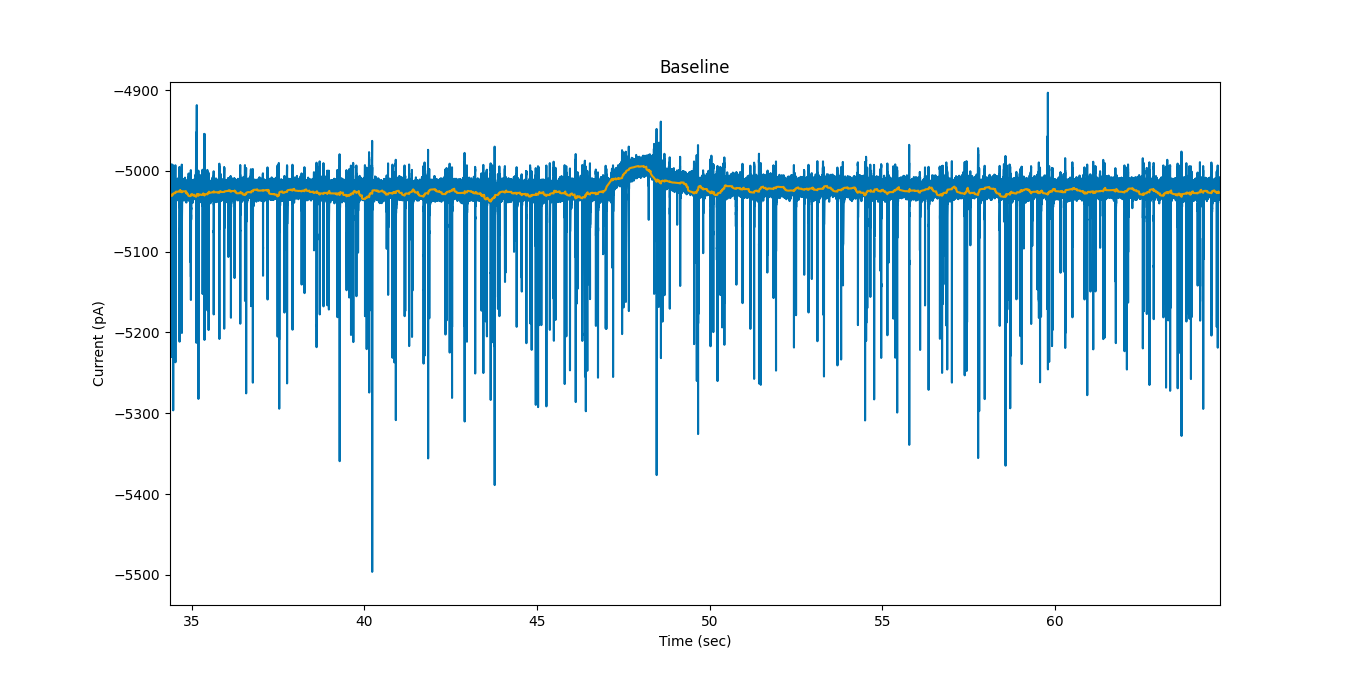
\includegraphics[width=3.49in]{imgs/PyNA_Dimer_Baseline.png}
  \caption{Nanopore signal with the detected baseline overlayed (window size = 30000) by PyNanoporeAnalyzer}
  \label{fig_4}
  \end{figure}

The application also provides supplementary block for subtracting two signals and flipping the result. The original signal and the detected baseline can be input to the \textit{SubtractAndFlip} class block to subtract the baseline from the signal. This makes the signal uniform allowing the use of a constant threshold value for detecting events. 

\subsection{Event Detection and Feature Extraction}
The amplitude threshold based detection method is used to detect translocation events in the recorded nanopore data. When the  current value crosses a predefined threshold, the application registers it as an event. It then tracks back to the sample where the signal deviated from the baseline. This is considered the start of the event. Each event includes the period from when the signal departed from the baseline level until it returns back to the baseline level. The \textit{EventDetect} class provides the implementation to detect all events in a given signal using this method. During event detection, the event maxima and event duration (baseline to baseline) is also recorded. The \textit{Event} class provides template to store the event trace along with it's features. Once the trace is extracted, various features in the events are extracted using the \textit{Event} class functions. The features extracted during this process are as follows:
\begin{list}{}{}
  \item Event amplitude (baseline to maxima)
  \item Event duration (baseline to baseline)
  \item Dwell time (full width at half maximum)
  \item Event rise time (baseline to maxima)
  \item Event fall time (maxima to baseline)
  \item Event integral (blocked charge)
\end{list}

All events are appended to the \textit{EventCollector} class object that creates a list and provides attributes to access particular feature for these events.

The threshold value can be a user specified fixed numeric value or can be calculated automatically by the software. The automatic threshold is selected as a multiple of the root mean square (RMS) of the signal noise level ($\sigma$), typically 5$\sigma$ \cite{plesaDataAnalysisMethods2015}. This multiplicative factor can be modified by the user.

\subsection{Visualisation}
There are numerous different data visualisation options provided with the PyNanoporeAnalyzer application which are as follows:

\subsubsection{Time domain plot}
The \textit{TimePlot} class provides block to plot a trace in the time domain. This is generally an amplitude vs time plot where the units of both axis and their resolution can be specified by the user.

\subsubsection{Frequency domain plot}
The \textit{FFTPlot} class provides block to plot a trace in the frequency domain. The block takes FFT arrays for the X-axis and Y-axis. A trace can be converted to frequency domain by using the \textit{sigFFT} class which returns the magnitude and frequency axis for the FFT of a signal.

\subsubsection{Histogram}
It is possible to plot Histograms by using the \textit{Histogram} class. The bin size for histograms can be set by user using the \textit{binWidth} parameter. This block also provides the option to fit the data to a Gaussian PDF and plots it over the histogram.

\subsubsection{Scatterplot}
Scatterplots are powerful visualization tools to look at data in two dimensions to find patterns, clusters and outliers. The \textit{Scatterplot} class can be invoked to display a scatterplot of any two event features which can be passed as input to this block.

\subsubsection{Density/Contour plot}
Density plot and contour plots are two alternatives ways to visualise data scatter. Similar to a scatterplot they show distribution of data points across two axes. They differ, however, in the presentation of this data. While scatterplots simply place a point for each event, density and contour plots change the colour of the point to indicate the concentration of points at a given location. This almost adds a third dimension to the data giving information about the population density. Contour plots go a step beyond and highlight contours around regions of same density, giving defined outlines to population groups. \textit{DensityPlot} and \textit{ContourPlot} classes provide blocks to generate such plots.  

\begin{lstlisting}[caption={Specifying Figure Options Example}]
Plot:
   class: FFTPlot
   parameters:
     figure_number: 2
     figure_options:
       title: Signal FFT
       ylabel: Magnitude
       xlabel: Frequency (Hz)
   inputs:
     - $Block3.output
\end{lstlisting}

All visualisation plots are generated using the python \textit{matplotlib} package. As such there are multiple figure options available to customize figures such as giving it Title, adding axis labels etc. These can be specified in the input file by nesting all options under the \textit{figure\_options} tag. Listing 2 shows example input for specifying figure options under parameters. It is also possible to provide figure number for each figure. This allows the user to overlay multiple plots by using the same figure number. However, care must be taken to ensure all overlayed plots have common axes. In order to ensure accessibility, a colour blind friendly palette is chosen as the default for all figures \cite{ichiharaColorUniversalDesign2008}.

\section{Performance Evaluation}
The performance of the PyNanoporeAnalyzer software was evaluated using the experimental recordings of supermolecular DNA nanostructures translocation events through nanopores. This data set was originally generated for another study at University of Leeds \cite{confederatNanoporeFingerprintingSupramolecular2022}. \footnote[1]{All data sets  were generated previously at University of Leeds for the study “Nanopore fingerprinting of supramolecular DNA nanostructures” by S. Confederat et. al. \cite{confederatNanoporeFingerprintingSupramolecular2022}} The original study used the Transalyzer software developed by Plesa and Dekker at TU Delft \cite{plesaDataAnalysisMethods2015} for analysis of the signal. In order ensure fair comparison, all parameters were chosen same as the original study where specified. Transalyzer's default settings were used for parameters which were not specified. 

Transalyzer uses a flow similar to that described in Fig. 1. The original study used an event detection threshold of 7$\sigma$. The input file used to configure PyNanoporeAnalyzer follows the following structure:
\begin{enumerate}{}{}
    \item {Load Data from ABF file.}
    \item {Butterworth LPF Filter: 2nd Order with 20KHz cutoff frequency.}
    \item {Baseline Detection: Moving window average with window size 30000.}
    \item {Subtract Baseline from original signal and flip for detecting peaks.}
    \item {Fit data histogram to Gaussian PDF to calculate $\sigma$. Set threshold to 7$\sigma$ level.}
    \item {Detect events and extract features}
\end{enumerate}
Multiple visualisation blocks have been added at various stages in the signal chain to allow better visualising of data.

\begin{figure}
  \centering
  \subfloat[][PyNanoporeAnalyzer]{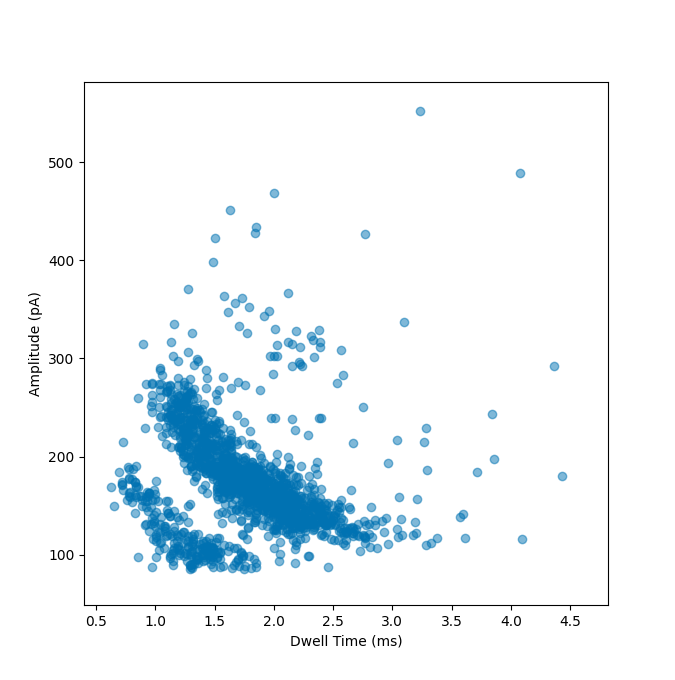
\includegraphics[width=1.74in]{imgs/PyNA_Dimer_Scatter.png}\label{fig_5a}}
  \subfloat[][Transalyzer]{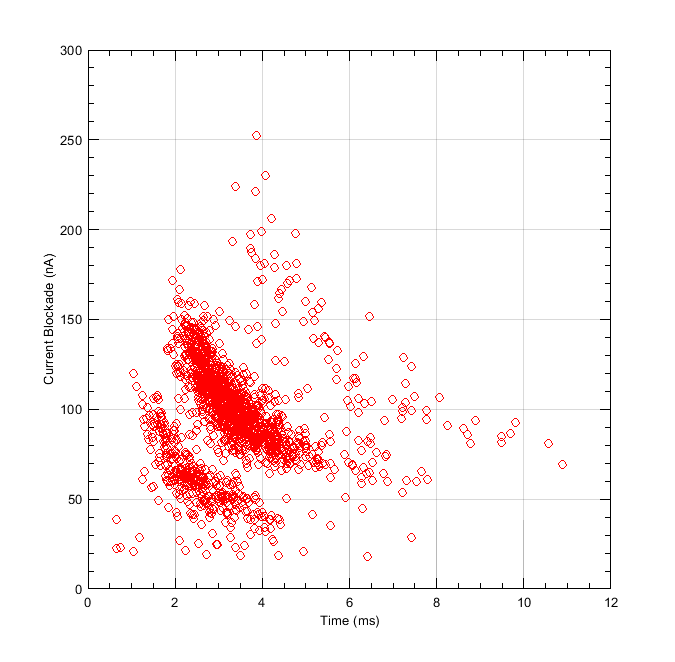
\includegraphics[width=1.74in]{imgs/TA_DimerScatter.png}\label{fig_5b}}
  \caption{Scatterplot comparison PyNanoporeAnalyzer vs Transalyzer}
\end{figure}

Fig. 5 presents scatterplots illustrating the relationship between amplitude and dwell time generated by PyNanoporeAnalyzer and Transalyzer. These plots were obtained from analyzing a recorded trace of dimer nanostructure translocations. Upon visual inspection, both software tools appear to produce comparable outcomes. Both software programs detected a similar number of events, with Transalyzer identifying 1566 events and PyNanoporeAnalyzer identifying 1521 events. However, a distinction can be observed in the peak amplitudes depicted in the scatterplot. Firstly, Transalyzer assumes the unit of measurement to be nanoamperes (nA), whereas for this specific dataset, it was measured in picoamperes (pA). Additionally, Transalyzer illustrates that the majority of event amplitudes are concentrated between 50nA to 150nA, whereas PyNanoporeAnalyzer displays a dominant range between 100pA to 300pA. Interestingly, the graph and readings presented by PyNanoporeAnalyzer exhibit a closer resemblance to those in the original research study \cite{confederatNanoporeFingerprintingSupramolecular2022}. Similar observations can also be made from fig. 6 which shows the histogram of event integrals.

\begin{figure}
  \centering
  \subfloat[][PyNanoporeAnalyzer]{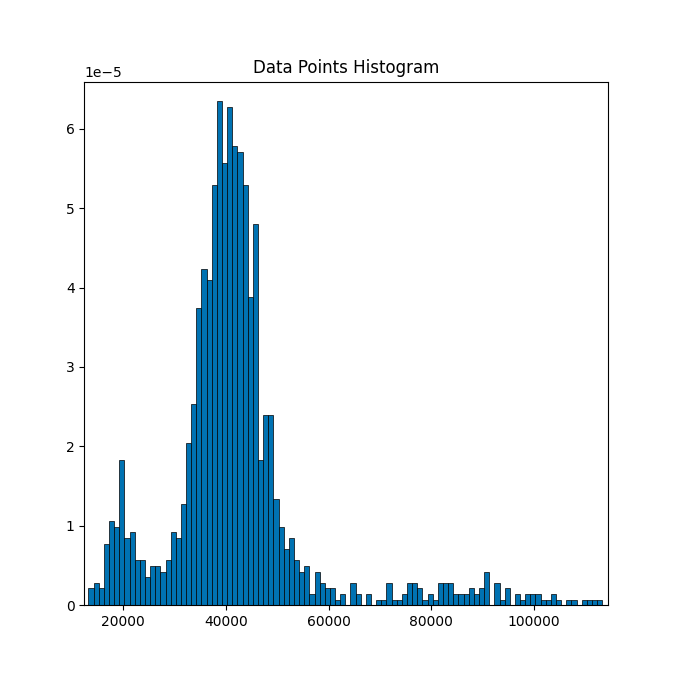
\includegraphics[width=1.74in]{imgs/PyNA_Dimer_Int.png}\label{fig_6a}}
  \subfloat[][Transalyzer]{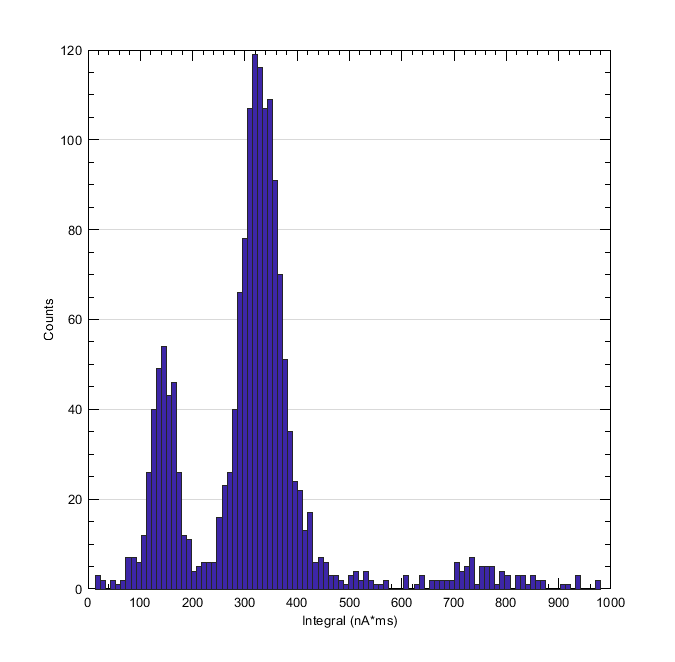
\includegraphics[width=1.74in]{imgs/TA_DimerInt.png}\label{fig_6b}}
  \caption{Integral histogram comparison PyNanoporeAnalyzer vs Transalyzer}
\end{figure}

\section{Conclusion}
\subsection{Project Evaluation: Aims, Objectives and Significant Technical Achievement}
PyNanoporeAnalyzer has successfully demonstrated remarkable capability in extracting event features from raw nanopore signals and presenting them through intuitive visualizations, which greatly aids in the analysis process. One of the primary challenges encountered during the development was accommodating the diverse nature of signals generated by solid-state nanopores. However, by adhering to a modular design approach, PyNanoporeAnalyzer has effectively addressed this obstacle. The application incorporates a comprehensive set of straightforward yet highly efficient algorithms for all stages of nanopore signal processing. It has also demostrated the ability to extract event features, offer multiple filtering options, and accommodate diverse signal types. Moreover, the modular architecture enables the integration of novel and improved algorithms without the need of modifications to existing functionality. This feature can be leveraged to combine algorithms developed for various applications, such as those used by MOSAIC \cite{forstaterMOSAICModularSingleMolecule2016}, SquiggleKit \cite{fergusonSquiggleKitToolkitManipulating2019}, and Transalyzer \cite{plesaDataAnalysisMethods2015}, thus further enhancing the capabilities of the software. PyNanoporeAnalyzer has been validated across multiple datasets, consisting of a wide range of analyte materials.

The PyNanoporeAnalyzer exhibits potential applications beyond the realm of nanopores in the biomedical signal processing domain. Notably, it can be adapted for Nano-Impact Single-Entity Electrochemistry Signals, which bear similarities to certain nanopore signals characterized by event spikes. Current research investigates the utilization of machine learning algorithms, such as template matching, for analyzing NIE signals \cite{zhaoAutomatedAnalysisNanoImpact2023}. Such algorithms can also be easily integrated within the existing framework provided by PyNanoporeAnalyzer.

\subsection{Future Work}
The existing set of algorithms implemented in PyNanoporeAnalyzer represents only a limited subset of methods employed for processing nanopore signals. In order to develop a more versatile and comprehensive tool for nanopore signal analysis, it is crucial to integrate additional algorithms such as ADEPT and CUSUM+ which are specifically designed for handling multi-state nanopore signals. The integration of complex filters, such as wavelet denoising filters and hidden Markov model-based denoising, can prove beneficial in handling signals with low SNR. Furthermore, incorporating improved baseline detection techniques discussed before \cite{plesaDataAnalysisMethods2015,varongchayakulSinglemoleculeProteinSensing2018} can enhance event detection accuracy. There is potential for incorporating further algorithms to extract more extensive event features from the nanopore signal as well. This can be achieved through the integration of statistical and machine learning methods, such as clustering, regression etc. The addition of more visualization tools, like an 'event viewer', which displays plots of each event alongside its detected features, would be valuable in providing better insights into the data.

It is worth noting that the current implementation of algorithms in the application may have certain inherent assumptions. This might have been influenced by the similarity of the experimental setup across the data sets used for testing. To mitigate this, future work should involve testing the software on various datasets with different analyte materials and experimental conditions. To ensure the software's robustness and reliability, extensive testing should be conducted to cover a wide range of scenarios.

\subsection{Reflections}
The initial design of the software, presented at the interim stage, contained some inherent flaws. The transition from a fixed signal chain to a modular approach helped to overcome these issues and facilitated in testing of individual algorithms. Moving from MATLAB to Python also enhanced control over the software's implementation through the utilization of various run-time polymorphism techniques, making the program more dynamic. The software ability to construct the signal chain at runtime based on inputs enables it to be used beyond nanopore signal processing domain. This adaptability allows the software to potentially process various signal types. Nevertheless, the currently implemented algorithm blocks are only suitable for analyzing a specific type of nanopore data. Expanding its features would require collaborative efforts from the community. Therefore, releasing the software under an open-source license is imperative. Given the right community support, the software has the potential to evolve into a powerful analysis tool.

\appendix
\noindent The code for the application is available on github at: https://github.com/sohamgokhale/PyNanoporeAnalyzer

\noindent The application has been tested with the following data sets:
\begin{enumerate}
  \item Confederat, Samuel (2022) Nanopore Fingerprinting of Supramolecular DNA Origami Nanostructures. University of Leeds. [Dataset] https://doi.org/10.5518/1198 (Data supporting Figures 1-5)
  \item Chau, Chalmers and Radford, Sheena and Hewitt, Eric and Actis, Paolo (2020) Dataset for Macromolecular crowding enhances the detection of DNA and proteins by a solid-state nanopore. University of Leeds. [Dataset] https://doi.org/10.5518/841
\end{enumerate}




\bibliography{Bibliography}
\bibliographystyle{IEEEtran}

\end{document}